\documentclass[10pt]{article}
\usepackage[a4paper,margin=18mm]{geometry}
\usepackage{amsmath,amssymb,booktabs,array,enumitem}
\usepackage[T1]{fontenc}\usepackage{lmodern}
\usepackage{tikz}\usetikzlibrary{shapes.gates.logic.US,positioning,arrows.meta,patterns,calc}
\usepackage[hidelinks]{hyperref}
\setlength{\parindent}{0pt}\setlength{\parskip}{4pt}
\setlength{\emergencystretch}{2em}
\newcommand{\VDD}{V_{DD}}
\newcommand{\mos}[4]{\begin{scope}[shift={(#1,#2)}]
\draw (0,.24)--(0,-.24);\draw (0,.20)--(.25,.20)--(.25,.5);
\draw (0,-.20)--(.25,-.20)--(.25,-.5);\draw (-.16,.23)--(-.16,-.23);
\ifnum#4=1\draw (-.26,0) circle (.06);\draw (-.75,0)--(-.32,0);\else\draw (-.75,0)--(-.16,0);\fi
\node[anchor=east,font=\scriptsize] at (-.76,0) {$#3$};\end{scope}}
\newcommand{\ground}[2]{\draw (#1,#2)--(#1,{#2-.12});\draw ({#1-.17},{#2-.12})--({#1+.17},{#2-.12});\draw ({#1-.11},{#2-.20})--({#1+.11},{#2-.20});}
\newcommand{\rail}[3]{\draw (#1,#2)--(#1,{#2+.14});\node[above,font=\scriptsize] at (#1,{#2+.14}) {$#3$};}

\newcommand{\hmos}[4]{\begin{scope}[shift={(#1,#2)}]
\draw(-.24,0)--(.24,0);\draw(-.2,0)--(-.2,-.25)--(-.5,-.25);\draw(.2,0)--(.2,-.25)--(.5,-.25);
\draw(-.23,.16)--(.23,.16);
\ifnum#4=1\draw(0,.26)circle(.06);\draw(0,.32)--(0,.75);\else\draw(0,.16)--(0,.75);\fi
\node[below,font=\scriptsize]at(0,-.32){#3};\end{scope}}
\begin{document}
\begin{center}{\Large\bfseries 2024 Final: independently checked solutions}\par EE3032 Introduction to VLSI Design, NCU\end{center}
The two original photographed exam pages and both supplied student answer sets were read. The original text, complement bars, circuit contacts and capacitance definitions govern this report; marks of 89 or 92 are only source provenance. Correct portions are retained after independent derivation. Incorrect charge-sharing cases, incomplete physical layout extraction and misread XOR equations are repaired. At the user's explicit choice, Q4 and Q6 present both the literal model and the classroom convention, with their incompatibilities visible. No process measurement is invented.

\section*{1. Brief answers (45 points)}
\begin{enumerate}[label=(\alph*),leftmargin=7mm,itemsep=7pt]
\item \textbf{Dynamic-logic power components.} Switching power from charging/discharging dynamic and output capacitances; clock-distribution/device-gate switching power; and short-circuit/keeper-contention power in evaluating/restoring gates. One useful accounting is $P_{dyn}=P_{data,sw}+P_{clock,sw}+P_{sc}$, with $P_{sw}=\alpha C V_{DD}^2f$. The clock usually switches every cycle even if data stays constant. Avoid double-counting clock capacitance in the first term. Leakage is static power and is not one of these requested dynamic components. The partial student set omits the short-circuit term.
\item \textbf{Improve IR-drop integrity.} Use wider and/or multiple parallel power metals with enough vias, lowering $R=\rho L/A$; and use more well-placed supply/ground pads or bumps with a denser grid, shortening current paths and spreading load. Both reduce $IR$ loss. Distributed decoupling additionally helps transient droop; it does not by itself remove steady DC resistive drop. Merely increasing an arbitrary logic delay is not a general power-grid fix.
\item \textbf{Latchup.} Parasitic pnp and npn bipolar devices in bulk CMOS form a positive-feedback PNPN/SCR path between VDD and VSS. Injected carriers or a transient can forward-bias a junction and trigger regeneration, creating a persistent low-impedance high-current path until current falls below its holding level. Guard rings with dense body/well ties collect injected carriers and reduce substrate/well resistance, lowering trigger susceptibility. A device ``being saturated'' is not the latchup mechanism. See the TI primary reference.
\item \textbf{NBTI.} A pMOS under negative gate-to-source bias, especially at elevated temperature, accumulates oxide/interface defects and trapped charge. Its threshold magnitude typically increases and drive degrades, increasing delay. Interface bond breaking/defect generation and charge trapping are the physical mechanisms; part of the degradation can recover when stress is removed. This is gradual bias/temperature-dependent aging, rather than instantaneous normal switching or a freely reversible threshold change.
\item \textbf{Two hold fixes.} Insert data-path delay buffers in an overly fast shift-register connection, increasing minimum data arrival time; or use a correctly phased lockup latch between skewed clock domains/segments, preventing the next data from racing through during the receiver's hold interval. The required inequality is $t_{launch}+t_{ccq}+t_{cd}\ge t_{capture}+t_{hold}$. Clock-skew balancing is another useful approach, but added delay must be placed with this inequality, not by guessing a buffer location.
\item \textbf{Two standard-cell layout requirements.} A common row height (or permitted integer-height family), and consistently aligned VDD/VSS rail positions so legal neighboring cells abut correctly. Widths normally follow the placement/site grid and all devices meet process rules. The student's height and fixed-rail ideas are retained.
\item \textbf{Reduce IO bounce.} Reduce package/supply-return inductance using additional short power/ground connections; and limit output-current slew, increasing appropriate rise/fall times to reduce $|L\,di/dt|$. Local decoupling may further help supply transients. A rise/fall-time reduction would generally increase bounce, not improve it.
\item \textbf{Reduce glitch power.} Balance reconvergent path delays by suitable buffering/sizing, reducing arrival mismatch; and use a functionally equivalent hazard-resistant logic cover/factoring (for example appropriate consensus terms for a static hazard). Simply declaring ``all gates serial'' does not guarantee the same function or eliminate glitches. Multi-input simultaneous transitions require their own hazard analysis.
\end{enumerate}
\newpage\subsection*{1(i). Differential pass-transistor implementation}
The original full-expression bar gives $f=\overline{x_1x_2+x_3}$, not $x_1x_2+x_3$. Use stable true/complement input rails and paired nMOS pass-selection networks:
\[
u_f=\bar x_2\bar x_3+x_2\,0,\qquad u_g=\bar x_2x_3+x_2\,1,
\qquad f=\bar x_1\bar x_3+x_1u_f,\qquad g=\bar x_1x_3+x_1u_g=\bar f.
\]
Both rails are restored by cross-coupled pMOS pull-ups. Each selected nMOS path passes a strong zero; the other pMOS, controlled by that zero rail, restores the selected weak high to VDD. The drawing assumes stable complementary input rails; if they are unavailable, three ordinary static CMOS input inverters add six MOS devices to this ten-device core. The two pass networks must be complementary for all eight data words; an uncomplemented f label would produce the wrong requested polarity.
% Requires TikZ only. Repeated terminal labels are electrical net names.
\providecommand{\auditmos}[4]{\begin{scope}[shift={(#1,#2)}]
\draw (0,.24)--(0,-.24);\draw (0,.20)--(.25,.20)--(.25,.5);
\draw (0,-.20)--(.25,-.20)--(.25,-.5);\draw (-.16,.23)--(-.16,-.23);
\ifnum#4=1\draw (-.26,0) circle (.06);\draw (-.75,0)--(-.32,0);
\else\draw (-.75,0)--(-.16,0);\fi
\node[anchor=east] at (-.76,0) {$#3$};\end{scope}}

\begin{center}
\begin{tikzpicture}[x=.72cm,y=.72cm,font=\scriptsize]
\auditmos{0}{0}{x_1}{0}
\draw (0.25,0.5)--(0.25,0.75) node[above] {$ \mathrm{f} $};
\draw (0.25,-0.5)--(0.25,-0.75) node[below] {$ \mathrm{uf} $};
\node[anchor=west] at (0.55,0) {$M_{1}$};
\auditmos{4.8}{0}{\bar x_1}{0}
\draw (5.05,0.5)--(5.05,0.75) node[above] {$ \mathrm{f} $};
\draw (5.05,-0.5)--(5.05,-0.75) node[below] {$ \bar x_3 $};
\node[anchor=west] at (5.35,0) {$M_{2}$};
\auditmos{9.6}{0}{x_2}{0}
\draw (9.85,0.5)--(9.85,0.75) node[above] {$ \mathrm{uf} $};
\draw (9.85,-0.5)--(9.85,-0.75) node[below] {$ V_{SS} $};
\node[anchor=west] at (10.15,0) {$M_{3}$};
\auditmos{14.4}{0}{\bar x_2}{0}
\draw (14.65,0.5)--(14.65,0.75) node[above] {$ \mathrm{uf} $};
\draw (14.65,-0.5)--(14.65,-0.75) node[below] {$ \bar x_3 $};
\node[anchor=west] at (14.95,0) {$M_{4}$};
\auditmos{0}{-2.5}{x_1}{0}
\draw (0.25,-2)--(0.25,-1.75) node[above] {$ \bar f $};
\draw (0.25,-3)--(0.25,-3.25) node[below] {$ \mathrm{ug} $};
\node[anchor=west] at (0.55,-2.5) {$M_{5}$};
\auditmos{4.8}{-2.5}{\bar x_1}{0}
\draw (5.05,-2)--(5.05,-1.75) node[above] {$ \bar f $};
\draw (5.05,-3)--(5.05,-3.25) node[below] {$ x_3 $};
\node[anchor=west] at (5.35,-2.5) {$M_{6}$};
\auditmos{9.6}{-2.5}{x_2}{0}
\draw (9.85,-2)--(9.85,-1.75) node[above] {$ \mathrm{ug} $};
\draw (9.85,-3)--(9.85,-3.25) node[below] {$ V_{DD} $};
\node[anchor=west] at (10.15,-2.5) {$M_{7}$};
\auditmos{14.4}{-2.5}{\bar x_2}{0}
\draw (14.65,-2)--(14.65,-1.75) node[above] {$ \mathrm{ug} $};
\draw (14.65,-3)--(14.65,-3.25) node[below] {$ x_3 $};
\node[anchor=west] at (14.95,-2.5) {$M_{8}$};
\auditmos{0}{-5}{\bar f}{1}
\draw (0.25,-4.5)--(0.25,-4.25) node[above] {$ \mathrm{f} $};
\draw (0.25,-5.5)--(0.25,-5.75) node[below] {$ V_{DD} $};
\node[anchor=west] at (0.55,-5) {$M_{9}$ (weak)};
\auditmos{4.8}{-5}{\mathrm{f}}{1}
\draw (5.05,-4.5)--(5.05,-4.25) node[above] {$ \bar f $};
\draw (5.05,-5.5)--(5.05,-5.75) node[below] {$ V_{DD} $};
\node[anchor=west] at (5.35,-5) {$M_{10}$ (weak)};
\end{tikzpicture}
\end{center}
\noindent\textbf{Q1(i),10MOS differential pass-transistor core}. $f=\overline{x_1x_2+x_3}$. The complementary inputs are provided; three static input inverters add six devices if required. The cross-coupled pMOS devices restore the high rail and must be suitably weak.
 Identically named terminals are connected. All nMOS bodies use $V_{SS}$ and all pMOS bodies use $V_{DD}$.

The executable checks all eight assignments and both rail networks. This is an ideal-switch functional check; fin/voltage/process sizing is not supplied by the exam.

\newpage\section*{2. Shared multioutput domino carry generation (5 points)}
\[
c_1=g_0+p_0c_0,\quad c_2=g_1+p_1c_1,
\quad c_3=g_2+p_2c_2.
\]
Each dynamic node $d_i$ is precharged high and drives an output inverter $c_i=\bar d_i$. Its evaluation network has a generate branch $g_{i-1}$ in parallel with the series propagate/carry branch $p_{i-1},c_{i-1}$. The three branches share one clocked evaluation footer; each dynamic node has its own precharge device and weak keeper. This is an explicit shared multioutput cell, with 22 core MOSFETs including output inverters/keepers. Stable input p/g/c0 values are established before evaluation; c1/c2 start at zero and can only rise, making same-clock cascading monotonic.
% Requires TikZ only. Repeated terminal labels are electrical net names.
\providecommand{\auditmos}[4]{\begin{scope}[shift={(#1,#2)}]
\draw (0,.24)--(0,-.24);\draw (0,.20)--(.25,.20)--(.25,.5);
\draw (0,-.20)--(.25,-.20)--(.25,-.5);\draw (-.16,.23)--(-.16,-.23);
\ifnum#4=1\draw (-.26,0) circle (.06);\draw (-.75,0)--(-.32,0);
\else\draw (-.75,0)--(-.16,0);\fi
\node[anchor=east] at (-.76,0) {$#3$};\end{scope}}

\begin{center}
\begin{tikzpicture}[x=.72cm,y=.72cm,font=\scriptsize]
\auditmos{0}{0}{\phi}{0}
\draw (0.25,0.5)--(0.25,0.75) node[above] {$ \mathrm{eval} $};
\draw (0.25,-0.5)--(0.25,-0.75) node[below] {$ V_{SS} $};
\node[anchor=west] at (0.55,0) {$M_{1}$};
\auditmos{4.8}{0}{\phi}{1}
\draw (5.05,0.5)--(5.05,0.75) node[above] {$ \mathrm{d1} $};
\draw (5.05,-0.5)--(5.05,-0.75) node[below] {$ V_{DD} $};
\node[anchor=west] at (5.35,0) {$M_{2}$};
\auditmos{9.6}{0}{\mathrm{g0}}{0}
\draw (9.85,0.5)--(9.85,0.75) node[above] {$ \mathrm{d1} $};
\draw (9.85,-0.5)--(9.85,-0.75) node[below] {$ \mathrm{eval} $};
\node[anchor=west] at (10.15,0) {$M_{3}$};
\auditmos{14.4}{0}{\mathrm{p0}}{0}
\draw (14.65,0.5)--(14.65,0.75) node[above] {$ \mathrm{d1} $};
\draw (14.65,-0.5)--(14.65,-0.75) node[below] {$ \mathrm{u0} $};
\node[anchor=west] at (14.95,0) {$M_{4}$};
\auditmos{0}{-2.5}{\mathrm{c0}}{0}
\draw (0.25,-2)--(0.25,-1.75) node[above] {$ \mathrm{u0} $};
\draw (0.25,-3)--(0.25,-3.25) node[below] {$ \mathrm{eval} $};
\node[anchor=west] at (0.55,-2.5) {$M_{5}$};
\auditmos{4.8}{-2.5}{\mathrm{c1}}{1}
\draw (5.05,-2)--(5.05,-1.75) node[above] {$ \mathrm{d1} $};
\draw (5.05,-3)--(5.05,-3.25) node[below] {$ V_{DD} $};
\node[anchor=west] at (5.35,-2.5) {$M_{6}$ (weak)};
\auditmos{9.6}{-2.5}{\mathrm{d1}}{1}
\draw (9.85,-2)--(9.85,-1.75) node[above] {$ \mathrm{c1} $};
\draw (9.85,-3)--(9.85,-3.25) node[below] {$ V_{DD} $};
\node[anchor=west] at (10.15,-2.5) {$M_{7}$};
\auditmos{14.4}{-2.5}{\mathrm{d1}}{0}
\draw (14.65,-2)--(14.65,-1.75) node[above] {$ \mathrm{c1} $};
\draw (14.65,-3)--(14.65,-3.25) node[below] {$ V_{SS} $};
\node[anchor=west] at (14.95,-2.5) {$M_{8}$};
\auditmos{0}{-5}{\phi}{1}
\draw (0.25,-4.5)--(0.25,-4.25) node[above] {$ \mathrm{d2} $};
\draw (0.25,-5.5)--(0.25,-5.75) node[below] {$ V_{DD} $};
\node[anchor=west] at (0.55,-5) {$M_{9}$};
\auditmos{4.8}{-5}{\mathrm{g1}}{0}
\draw (5.05,-4.5)--(5.05,-4.25) node[above] {$ \mathrm{d2} $};
\draw (5.05,-5.5)--(5.05,-5.75) node[below] {$ \mathrm{eval} $};
\node[anchor=west] at (5.35,-5) {$M_{10}$};
\auditmos{9.6}{-5}{\mathrm{p1}}{0}
\draw (9.85,-4.5)--(9.85,-4.25) node[above] {$ \mathrm{d2} $};
\draw (9.85,-5.5)--(9.85,-5.75) node[below] {$ \mathrm{u1} $};
\node[anchor=west] at (10.15,-5) {$M_{11}$};
\auditmos{14.4}{-5}{\mathrm{c1}}{0}
\draw (14.65,-4.5)--(14.65,-4.25) node[above] {$ \mathrm{u1} $};
\draw (14.65,-5.5)--(14.65,-5.75) node[below] {$ \mathrm{eval} $};
\node[anchor=west] at (14.95,-5) {$M_{12}$};
\auditmos{0}{-7.5}{\mathrm{c2}}{1}
\draw (0.25,-7)--(0.25,-6.75) node[above] {$ \mathrm{d2} $};
\draw (0.25,-8)--(0.25,-8.25) node[below] {$ V_{DD} $};
\node[anchor=west] at (0.55,-7.5) {$M_{13}$ (weak)};
\auditmos{4.8}{-7.5}{\mathrm{d2}}{1}
\draw (5.05,-7)--(5.05,-6.75) node[above] {$ \mathrm{c2} $};
\draw (5.05,-8)--(5.05,-8.25) node[below] {$ V_{DD} $};
\node[anchor=west] at (5.35,-7.5) {$M_{14}$};
\auditmos{9.6}{-7.5}{\mathrm{d2}}{0}
\draw (9.85,-7)--(9.85,-6.75) node[above] {$ \mathrm{c2} $};
\draw (9.85,-8)--(9.85,-8.25) node[below] {$ V_{SS} $};
\node[anchor=west] at (10.15,-7.5) {$M_{15}$};
\auditmos{14.4}{-7.5}{\phi}{1}
\draw (14.65,-7)--(14.65,-6.75) node[above] {$ \mathrm{d3} $};
\draw (14.65,-8)--(14.65,-8.25) node[below] {$ V_{DD} $};
\node[anchor=west] at (14.95,-7.5) {$M_{16}$};
\auditmos{0}{-10}{\mathrm{g2}}{0}
\draw (0.25,-9.5)--(0.25,-9.25) node[above] {$ \mathrm{d3} $};
\draw (0.25,-10.5)--(0.25,-10.75) node[below] {$ \mathrm{eval} $};
\node[anchor=west] at (0.55,-10) {$M_{17}$};
\auditmos{4.8}{-10}{\mathrm{p2}}{0}
\draw (5.05,-9.5)--(5.05,-9.25) node[above] {$ \mathrm{d3} $};
\draw (5.05,-10.5)--(5.05,-10.75) node[below] {$ \mathrm{u2} $};
\node[anchor=west] at (5.35,-10) {$M_{18}$};
\auditmos{9.6}{-10}{\mathrm{c2}}{0}
\draw (9.85,-9.5)--(9.85,-9.25) node[above] {$ \mathrm{u2} $};
\draw (9.85,-10.5)--(9.85,-10.75) node[below] {$ \mathrm{eval} $};
\node[anchor=west] at (10.15,-10) {$M_{19}$};
\auditmos{14.4}{-10}{\mathrm{c3}}{1}
\draw (14.65,-9.5)--(14.65,-9.25) node[above] {$ \mathrm{d3} $};
\draw (14.65,-10.5)--(14.65,-10.75) node[below] {$ V_{DD} $};
\node[anchor=west] at (14.95,-10) {$M_{20}$ (weak)};
\auditmos{0}{-12.5}{\mathrm{d3}}{1}
\draw (0.25,-12)--(0.25,-11.75) node[above] {$ \mathrm{c3} $};
\draw (0.25,-13)--(0.25,-13.25) node[below] {$ V_{DD} $};
\node[anchor=west] at (0.55,-12.5) {$M_{21}$};
\auditmos{4.8}{-12.5}{\mathrm{d3}}{0}
\draw (5.05,-12)--(5.05,-11.75) node[above] {$ \mathrm{c3} $};
\draw (5.05,-13)--(5.05,-13.25) node[below] {$ V_{SS} $};
\node[anchor=west] at (5.35,-12.5) {$M_{22}$};
\end{tikzpicture}
\end{center}
\noindent\textbf{Q2,22MOS shared-footer carry generator}. One clocked nMOS footer is shared by all three carry stages. The three positive inverter outputs drive later transistor gates, not later dynamic-node channels. $c_0,p_i,g_i$ remain stable through evaluation.
 Identically named terminals are connected. All nMOS bodies use $V_{SS}$ and all pMOS bodies use $V_{DD}$.

The student's three separately footed domino stages implement the recurrence, but a shared footer makes the requested multioutput structure explicit. Do not connect raw dynamic drain nodes by bidirectional propagate pass devices without additional constraints: independent p/g words can back-discharge a previously false carry. All 128 independent p/g/c0 combinations are checked; no unprinted p/g exclusivity constraint is used.

\newpage\section*{3. Dynamic gates, sharing and retention (15 points)}
\subsection*{(a) Read the middle clock and output bar}
The left n-type dynamic gate has pull-down function
\[F=AB+C(A+B),\qquad Z=\bar F\ \text{during evaluation}.\]
The middle output is printed $\bar Y$; call that physical node $Y_b$ to distinguish the label from its Boolean value. Its upper pMOS and lower footer use $\bar\phi$, not Z. For $\phi=0$, the left gate precharges Z high while the middle stage evaluates low. For $\phi=1$, the middle pMOS precharges $Y_b$ high and its footer is off, independent of F. Thus it does not evaluate the first gate's data in the intended evaluation phase. The right p-type branch correctly accepts falling Z and gives X=F. The middle clock overbar touches its gate wire in this photograph; a barred clock is the selected transcription, but the touching stroke cannot establish that glyph definitively. If that touching stroke instead denotes only the wire and the label is unbarred, the middle becomes a same-phase n-dynamic cascade: an initially high Z can discharge it before Z falls, and it cannot recharge during evaluation. It is still invalid, and the static repair below works for either clock reading.

One valid repair makes the middle stage a static inverter: \textbf{rewire the upper pMOS gate from the clock to Z, and remove the footer} (or tie it permanently on). Both inverter gates then use Z. It resets $Y_b=0$ while Z is precharged high and gives $Y_b=F$ in evaluation. Keep the right p-type branch on raw Z. The prompt does not impose another Boolean output specification; this repair chooses $Y_b=X=F$.
\begin{center}\begin{tikzpicture}[scale=.82,font=\small]
\mos{2}{4}{\phi}{1}\rail{2.25}{4.5}{V_{DD}}
\draw(.25,3.5)--(3.25,3.5);\fill(2.25,3.5)circle(1.5pt);\node[above]at(1.3,3.5){$Z$};
\mos{0}{3}{A}{0}\mos{0}{2}{B}{0}\mos{3}{3}{C}{0}\mos{2}{2}{A}{0}\mos{4}{2}{B}{0}
\draw(2.25,2.5)--(4.25,2.5);\fill(3.25,2.5)circle(1.5pt);\node[above]at(3.7,2.5){$y$};\node[right]at(.25,2.5){$x$};
\draw(.25,1.5)--(4.25,1.5);\mos{2}{1}{\phi}{0}\ground{2.25}{.5}
\mos{7}{3.8}{Z}{1}\rail{7.25}{4.3}{V_{DD}}\mos{7}{2.5}{Z}{0}\draw(7.25,3)--(7.25,3.3);\draw(7.25,3.15)--(8.25,3.15)node[pos=.55,above]{$\bar Y$};
\ground{7.25}{2}
\mos{10}{4}{\bar\phi}{1}\rail{10.25}{4.5}{V_{DD}}\mos{10}{3}{Z}{1}\mos{10}{1.8}{\bar\phi}{0}\draw(10.25,2.3)--(10.25,2.5)--(11.1,2.5)node[right]{$X$};\ground{10.25}{1.3}
\draw(2.25,3.5)--(5.75,3.5);\draw(5.75,2.5)--(5.75,3.8)--(6.25,3.8);\draw(5.75,2.5)--(6.25,2.5);\fill(5.75,3.5)circle(1.5pt);\draw(5.75,3.5)--(9,3.5)--(9,3)--(9.25,3);
\end{tikzpicture}\end{center}
The student's alternate inserts an inverter between Z and the middle nMOS and changes the middle clock to $\phi$. That is also valid n-type domino: its rising F input discharges $Y_b$, giving $Y_b=\bar F$ after evaluation. Retain it as a valid alternate with this explicit polarity; add an output inverter only if the selected specification requires F. ``Dynamic gates cannot cascade'' is too broad: phase and input monotonicity determine validity.

\subsection*{(b) Enumerate sharing-only states before adding capacitances}
Z connects three drain capacitances (precharge pMOS and top A/C nMOS) and three driven gate capacitances (the static middle inverter's two gates and right input pMOS gate):
\[C_Z=3C_d+3C_g=3.3\,\mathrm{fF}.\]
Treat the supplied internal-node parasitic capacitances as total nodal values. In an F=0 state, Z can share with x only at ABC=100, or with y only at ABC=001. It cannot reach both x and y without also opening a complete ground-discharge path (F=1).
\begin{center}\begin{tabular}{cccc}\toprule ABC&Connected floating node&Worst discharged-node share&Result\\\midrule
100&x, $1.3$ fF&$V_Z=3.3/(3.3+1.3)V_{DD}=0.71739V_{DD}$&above $V_{DD}/2$\\
001&y, $1.1$ fF&$V_Z=3.3/(3.3+1.1)V_{DD}=0.75V_{DD}$&above $V_{DD}/2$\\\bottomrule\end{tabular}\end{center}
Thus the stated half-supply switching criterion is not crossed by these sharing-only events. The student's ABC=101 case is a real C--A pull-down path; its F=1 voltage must discharge, so a combined $C_x+C_y$ charge-sharing ratio is not a valid argument for that word. If the source's nodal values were instead additional wire capacitances, adding the corresponding diffusion terms still leaves both sharing-only ratios above one half; the saved alternative is labeled, not silently substituted.

\subsection*{(c) Longer clock intervals require retention}
With precharge/evaluation clock held for a long time, a floating dynamic rail can leak across a logic threshold; purely capacitive storage does not provide indefinite retention. Add a weak pMOS feedback keeper from VDD to Z, controlled by static $Y_b=\bar Z$. Add a weak nMOS keeper from X to VSS, controlled by a static inverter's $\bar X$. These hold the otherwise floating high Z and low X states respectively. The evaluating network must overcome its weak keeper until the feedback disables it; arbitrary device strengths cannot be inferred from the prompt.
\begin{center}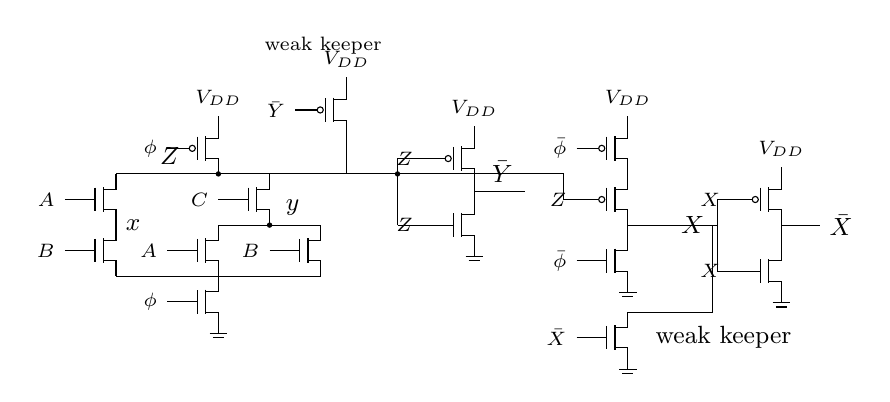
\begin{tikzpicture}[scale=.65,font=\small]
\mos{2}{4}{\phi}{1}\rail{2.25}{4.5}{V_{DD}}
\draw(.25,3.5)--(3.25,3.5);\fill(2.25,3.5)circle(1.5pt);\node[above]at(1.3,3.5){$Z$};
\mos{0}{3}{A}{0}\mos{0}{2}{B}{0}\mos{3}{3}{C}{0}\mos{2}{2}{A}{0}\mos{4}{2}{B}{0}
\draw(2.25,2.5)--(4.25,2.5);\fill(3.25,2.5)circle(1.5pt);\node[above]at(3.7,2.5){$y$};\node[right]at(.25,2.5){$x$};
\draw(.25,1.5)--(4.25,1.5);\mos{2}{1}{\phi}{0}\ground{2.25}{.5}
\mos{7}{3.8}{Z}{1}\rail{7.25}{4.3}{V_{DD}}\mos{7}{2.5}{Z}{0}\draw(7.25,3)--(7.25,3.3);\draw(7.25,3.15)--(8.25,3.15)node[pos=.55,above]{$\bar Y$};
\ground{7.25}{2}
\mos{10}{4}{\bar\phi}{1}\rail{10.25}{4.5}{V_{DD}}\mos{10}{3}{Z}{1}\mos{10}{1.8}{\bar\phi}{0}\draw(10.25,2.3)--(10.25,2.5)--(11.1,2.5)node[right]{$X$};\ground{10.25}{1.3}
\draw(2.25,3.5)--(5.75,3.5);\draw(5.75,2.5)--(5.75,3.8)--(6.25,3.8);\draw(5.75,2.5)--(6.25,2.5);\fill(5.75,3.5)circle(1.5pt);\draw(5.75,3.5)--(9,3.5)--(9,3)--(9.25,3);
\mos{4.5}{4.75}{\bar Y}{1}\rail{4.75}{5.25}{V_{DD}}\draw(4.75,4.25)--(4.75,3.5);\node[above,font=\scriptsize]at(4.3,5.65){weak keeper};
\mos{10}{.3}{\bar X}{0}\draw(10.25,.8)--(11.9,.8)--(11.9,2.5)--(10.25,2.5);\ground{10.25}{-.2}\node[right]at(10.6,.3){weak keeper};
\mos{13}{3}{X}{1}\mos{13}{1.6}{X}{0}\rail{13.25}{3.5}{V_{DD}}\draw(13.25,2.1)--(13.25,2.5)--(14.0,2.5)node[right]{$\bar X$};\ground{13.25}{1.1}
\draw(11.1,2.5)--(12,2.5);\draw(12,1.6)--(12,3)--(12.25,3);\draw(12,1.6)--(12.25,1.6);
\end{tikzpicture}\end{center}
This addresses ideal retention and practical leakage over a designed interval. Actual unlimited stopping time and noise margins require device/leakage/keeper sizing not supplied by the exam. The complementary X-control inverter is shown explicitly; adding only a left-rail keeper would omit the right p-type storage rail.

\newpage\section*{4. Schmitt trigger: convention and literal load (11 points)}
\subsection*{(a) Thresholds and classroom sizing}
The waveform requires rising-input threshold $V_T^+=1.0$ V and falling-input threshold $V_T^-=0.5$ V. In the supplied resistance approximation, the internal n-stack node before switching is $u_n=V_T^+-V_{tn}=0.8$ V and the p-stack node is $u_p=V_T^-+|V_{tp}|=0.7$ V. Hence
\[
\frac{R_{N1}}{R_{N1}+R_{N3}}=\frac{0.8}{1.5}=\frac8{15},\quad
\frac{R_{P3}}{R_{P1}+R_{P3}}=\frac{0.7}{1.5}=\frac7{15}.
\]
The width ratios are $W_{N3}/W_{N1}=8/7$ and $W_{P3}/W_{P1}=8/7$. With all lengths 40 nm, one classroom fixed-output-load-C convention yields:
\begin{center}\begin{tabular}{crr}\toprule Device&Width (nm)&ON resistance relative R\\\midrule
N1&160&1\\N2&80&2\\N3&$1280/7\simeq182.857$&$7/8$\\
P1&320&1\\P2&160&2\\P3&$2560/7\simeq365.714$&$7/8$\\\bottomrule\end{tabular}\end{center}
Each main pull-up/down path has resistance 3R, so if the output load is \emph{assumed independently equal to C}, $t_r=t_f=3RC$. This is the marked student's resistance-only convention, not a consequence of the literal capacitance definition.

\subsection*{Literal output gate capacitance: target is infeasible}
The exam defines C as \emph{N1's gate capacitance} and only discards drain capacitance. Output drives N3 and P3 gates, so the above widths give
\[C_{out}=\frac{W_{N3}+W_{P3}}{160}C=\frac{24}{7}C,
\qquad t_r=t_f=\frac{72}{7}RC\simeq10.286RC.\]
More generally, write $W_{P1}=160a$, $W_{N2}=160b$, $W_{P2}=160c$ nm. The threshold ratios enforce $W_{N3}=160(8/7)$ and $W_{P3}=160(8a/7)$. Then
\[
\frac{t_f}{RC}=\frac8{7}(1+a)(1+1/b),\qquad
\frac{t_r}{RC}=\frac{16}{7}(1+a)(1/a+1/c).
\]
Even letting b and c approach infinity cannot make the jointly optimized maximum smaller than $24/7\,RC\simeq3.429RC$, attained as an infimum at a=2. Therefore the literal gate-capacitance model has \textbf{no sizing satisfying both 3RC targets}. The fixed-C convention and the literal result are shown separately at the user's request. The RC prefactor convention is stated; no unsupported physical rise/fall measurement is reported.

\subsection*{(b) Switches increase feedback}
Turning on the switches connects P4/N4 to the output-controlled feedback devices in parallel, strengthening both feedback paths. Under the intended disabled-extra-device OFF baseline, $V_T^+$ rises and $V_T^-$ falls, increasing hysteresis and noise tolerance. Assuming the extra feedback devices match P3/N3 in width gives an illustrative ON case:
\[V_T^+=143/115\simeq1.24348\,\mathrm V,\quad
V_T^-=59/230\simeq0.25652\,\mathrm V,\quad
V_H=227/230\simeq0.98696\,\mathrm V>0.5\,\mathrm V.\]
Stronger feedback increases the auxiliary conduction current for the same input/output bias; its simple resistance estimate changes from $V_{DD}/(R_1+R_3)$ to $V_{DD}/(R_1+R_3/2)$, an increase by factor $30/23$. The student's minus sign in a series-resistance denominator is incorrect. Cycle-averaged short-circuit power also depends on input slew, operating waveform and sizing; without these, the increased-current classroom expectation is not an unconditional numerical power claim.

The original open switches leave P4/N4 gates floating, without drawn OFF clamps. A practical controllable design must clamp P4's gate high and N4's gate low while disabled (or specify stored gate charge). The source symbol alone cannot guarantee that opening a switch makes those devices off.

\newpage\section*{5. Extract every physical transistor (10 points)}
The seven poly crossings of each active strip create \textbf{14 physical MOSFETs}. Four are intentionally off isolation devices: two pMOS gates tied VDD and two nMOS gates tied VSS. They cannot be omitted when drawing the literal layout's complete transistor schematic.
\begin{center}\begin{tabular}{cl}\toprule Strip&Diffusion-node sequence left to right\\\midrule
pMOS&VDD, x, VDD, p1, p2, w, VDD, z\\
nMOS&VSS, x, VSS, w, VSS, w, VSS, z\\\midrule
Strip&Gate sequence left to right\\\midrule
pMOS&a, VDD, x, b, c, VDD, w\\
nMOS&a, VSS, x, b, c, VSS, w\\\bottomrule\end{tabular}\end{center}
Only black contact markers join metal to poly/diffusion. Uncontacted layer crossings stay insulated. The internal p1/p2 source/drain contacts do not connect to the VDD rail; treating those as power contacts would destroy the series pull-up.
% Requires TikZ only. Repeated terminal labels are electrical net names.
\providecommand{\auditmos}[4]{\begin{scope}[shift={(#1,#2)}]
\draw (0,.24)--(0,-.24);\draw (0,.20)--(.25,.20)--(.25,.5);
\draw (0,-.20)--(.25,-.20)--(.25,-.5);\draw (-.16,.23)--(-.16,-.23);
\ifnum#4=1\draw (-.26,0) circle (.06);\draw (-.75,0)--(-.32,0);
\else\draw (-.75,0)--(-.16,0);\fi
\node[anchor=east] at (-.76,0) {$#3$};\end{scope}}

\begin{center}
\begin{tikzpicture}[x=.72cm,y=.72cm,font=\scriptsize]
\auditmos{0}{0}{a}{1}
\draw (0.25,0.5)--(0.25,0.75) node[above] {$ V_{DD} $};
\draw (0.25,-0.5)--(0.25,-0.75) node[below] {$ \mathrm{x} $};
\node[anchor=west] at (0.55,0) {$M_{1}$};
\auditmos{4.8}{0}{V_{DD}}{1}
\draw (5.05,0.5)--(5.05,0.75) node[above] {$ \mathrm{x} $};
\draw (5.05,-0.5)--(5.05,-0.75) node[below] {$ V_{DD} $};
\node[anchor=west] at (5.35,0) {$M_{2}$};
\auditmos{9.6}{0}{\mathrm{x}}{1}
\draw (9.85,0.5)--(9.85,0.75) node[above] {$ V_{DD} $};
\draw (9.85,-0.5)--(9.85,-0.75) node[below] {$ \mathrm{p1} $};
\node[anchor=west] at (10.15,0) {$M_{3}$};
\auditmos{14.4}{0}{b}{1}
\draw (14.65,0.5)--(14.65,0.75) node[above] {$ \mathrm{p1} $};
\draw (14.65,-0.5)--(14.65,-0.75) node[below] {$ \mathrm{p2} $};
\node[anchor=west] at (14.95,0) {$M_{4}$};
\auditmos{0}{-2.5}{c}{1}
\draw (0.25,-2)--(0.25,-1.75) node[above] {$ \mathrm{p2} $};
\draw (0.25,-3)--(0.25,-3.25) node[below] {$ \mathrm{w} $};
\node[anchor=west] at (0.55,-2.5) {$M_{5}$};
\auditmos{4.8}{-2.5}{V_{DD}}{1}
\draw (5.05,-2)--(5.05,-1.75) node[above] {$ \mathrm{w} $};
\draw (5.05,-3)--(5.05,-3.25) node[below] {$ V_{DD} $};
\node[anchor=west] at (5.35,-2.5) {$M_{6}$};
\auditmos{9.6}{-2.5}{\mathrm{w}}{1}
\draw (9.85,-2)--(9.85,-1.75) node[above] {$ V_{DD} $};
\draw (9.85,-3)--(9.85,-3.25) node[below] {$ \mathrm{z} $};
\node[anchor=west] at (10.15,-2.5) {$M_{7}$};
\auditmos{14.4}{-2.5}{a}{0}
\draw (14.65,-2)--(14.65,-1.75) node[above] {$ V_{SS} $};
\draw (14.65,-3)--(14.65,-3.25) node[below] {$ \mathrm{x} $};
\node[anchor=west] at (14.95,-2.5) {$M_{8}$};
\auditmos{0}{-5}{V_{SS}}{0}
\draw (0.25,-4.5)--(0.25,-4.25) node[above] {$ \mathrm{x} $};
\draw (0.25,-5.5)--(0.25,-5.75) node[below] {$ V_{SS} $};
\node[anchor=west] at (0.55,-5) {$M_{9}$};
\auditmos{4.8}{-5}{\mathrm{x}}{0}
\draw (5.05,-4.5)--(5.05,-4.25) node[above] {$ V_{SS} $};
\draw (5.05,-5.5)--(5.05,-5.75) node[below] {$ \mathrm{w} $};
\node[anchor=west] at (5.35,-5) {$M_{10}$};
\auditmos{9.6}{-5}{b}{0}
\draw (9.85,-4.5)--(9.85,-4.25) node[above] {$ \mathrm{w} $};
\draw (9.85,-5.5)--(9.85,-5.75) node[below] {$ V_{SS} $};
\node[anchor=west] at (10.15,-5) {$M_{11}$};
\auditmos{14.4}{-5}{c}{0}
\draw (14.65,-4.5)--(14.65,-4.25) node[above] {$ V_{SS} $};
\draw (14.65,-5.5)--(14.65,-5.75) node[below] {$ \mathrm{w} $};
\node[anchor=west] at (14.95,-5) {$M_{12}$};
\auditmos{0}{-7.5}{V_{SS}}{0}
\draw (0.25,-7)--(0.25,-6.75) node[above] {$ \mathrm{w} $};
\draw (0.25,-8)--(0.25,-8.25) node[below] {$ V_{SS} $};
\node[anchor=west] at (0.55,-7.5) {$M_{13}$};
\auditmos{4.8}{-7.5}{\mathrm{w}}{0}
\draw (5.05,-7)--(5.05,-6.75) node[above] {$ V_{SS} $};
\draw (5.05,-8)--(5.05,-8.25) node[below] {$ \mathrm{z} $};
\node[anchor=west] at (5.35,-7.5) {$M_{14}$};
\end{tikzpicture}
\end{center}
\noindent\textbf{Q5,all14physical MOS crossings}. Four rail-tied isolation devices are always off. The functional10-device circuit is $x=\bar a$, $w=\overline{x+b+c}$, $z=\bar w=\bar a+b+c$. Use the lowercase layout input labels a,b,c in the accompanying diagram.
 Identically named terminals are connected. All nMOS bodies use $V_{SS}$ and all pMOS bodies use $V_{DD}$.

The ten functional devices reduce to INV(a), NOR(x,b,c), and INV(w), with $x=\bar a$, $w=\overline{x+b+c}$ and $z=x+b+c=\bar a+b+c$. The student's functional NOR sketch is valid after excluding the off isolation devices, but its 10-device picture is not the full 14-crossing extraction requested. All eight a/b/c words and rail-exclusivity states are checked against the full physical graph.

\newpage\section*{6. Sequential circuit: preserve the NOR (24 points)}
Let A, B, C be the outputs of R1, R2, R3, and define $u=A\oplus B$. The original middle gates are NAND(A,B) and NAND(u,C), followed by a \emph{NOR}, while the R5 path has a second XOR:
\[
Y_1=\overline{\overline{AB}+\overline{uC}}=AB\,uC=0,
\qquad Y_2=u\oplus C=A\oplus B\oplus C.
\]
The source is not the conventional carry adder with a final NAND; substituting that NAND changes its function. The student adds an extra u in the parity expression and incorrectly reduces Y2 to C. Although Y1 is steady zero, reconvergent unequal delays can create a pulse; structural timing analysis of the original gates still bounds settling before capture.

\subsection*{(a) Setup inequality and two approved skew readings}
For clock arrivals L at launch and K at capture,
\[T\ge L+t_{pcq}+t_{pd}+t_{setup}-K.\]
The longest physical combinational path to each output is 2 ns. With $t_{pcq}=t_{setup}=0.2$ ns, zero-skew setup time is 2.4 ns.
\begin{center}\begin{tabular}{lrrr}\toprule Reading&R4 bound(ns)&R5 bound(ns)&Setup maximum frequency\\\midrule
Literal positive R4-capture delay +0.6&1.8&2.4&416.667 MHz\\
Adverse R4 skew -0.6 classroom convention&3.0&2.4&333.333 MHz\\\bottomrule\end{tabular}\end{center}
The literal reading already permits 400 MHz, so the source's wording ``boosted to 400MHz'' is inconsistent with that reading. The student's 333.333MHz uses adverse skew instead of the positive capture delay pictured. Both are presented as explicitly distinct interpretations; no hidden sign reversal repairs the original figure.

\subsection*{(b) Clock buffering at the 400MHz target}
Two 0.3ns inverters form a 0.6ns noninverting buffer. \textbf{Literal figure:} leave R4's existing 0.6ns branch and add a two-inverter pair to every R1/R2/R3 and R5 branch, making all arrivals0.6ns. \textbf{Adverse interpretation:} choose physical arrivals $(R1,R2,R3,R4,R5)=(0.6,0.6,0.6,0,0.6)$ns, then add the pair only on R4's shorter branch. Both balanced trees have setup bound2.4ns, safely within the requested2.5ns period. They permit416.667MHz under the same ideal setup model;400MHz is an achieved target, not the new exact maximum.
\begin{center}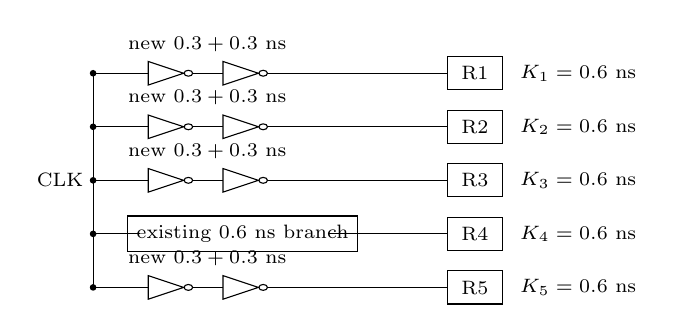
\begin{tikzpicture}[x=1cm,y=.68cm,font=\scriptsize]
\draw(0,0)--(0,4);\node[left]at(0,2){CLK};
\draw(0,4)--(.7,4);\draw(.7,3.78)--(.7,4.22)--(1.15,4)--cycle;\draw(1.21,4)circle(.055);\draw(1.27,4)--(1.65,4);\draw(1.65,3.78)--(1.65,4.22)--(2.1,4)--cycle;\draw(2.16,4)circle(.055);\draw(2.22,4)--(4.5,4);\node[above]at(1.45,4.22){new $0.3+0.3$ ns};
\node[draw,minimum width=.7cm,minimum height=.42cm]at(4.85,4){R1};\node[right]at(5.3,4){$K_{1}=0.6$ ns};\fill(0,4)circle(1.2pt);
\draw(0,3)--(.7,3);\draw(.7,2.78)--(.7,3.22)--(1.15,3)--cycle;\draw(1.21,3)circle(.055);\draw(1.27,3)--(1.65,3);\draw(1.65,2.78)--(1.65,3.22)--(2.1,3)--cycle;\draw(2.16,3)circle(.055);\draw(2.22,3)--(4.5,3);\node[above]at(1.45,3.22){new $0.3+0.3$ ns};
\node[draw,minimum width=.7cm,minimum height=.42cm]at(4.85,3){R2};\node[right]at(5.3,3){$K_{2}=0.6$ ns};\fill(0,3)circle(1.2pt);
\draw(0,2)--(.7,2);\draw(.7,1.78)--(.7,2.22)--(1.15,2)--cycle;\draw(1.21,2)circle(.055);\draw(1.27,2)--(1.65,2);\draw(1.65,1.78)--(1.65,2.22)--(2.1,2)--cycle;\draw(2.16,2)circle(.055);\draw(2.22,2)--(4.5,2);\node[above]at(1.45,2.22){new $0.3+0.3$ ns};
\node[draw,minimum width=.7cm,minimum height=.42cm]at(4.85,2){R3};\node[right]at(5.3,2){$K_{3}=0.6$ ns};\fill(0,2)circle(1.2pt);
\draw(0,1)--(.6,1);\node[draw,minimum width=2.2cm,minimum height=.28cm]at(1.9,1){existing 0.6 ns branch};\draw(3.0,1)--(4.5,1);
\node[draw,minimum width=.7cm,minimum height=.42cm]at(4.85,1){R4};\node[right]at(5.3,1){$K_{4}=0.6$ ns};\fill(0,1)circle(1.2pt);
\draw(0,0)--(.7,0);\draw(.7,-0.22)--(.7,0.22)--(1.15,0)--cycle;\draw(1.21,0)circle(.055);\draw(1.27,0)--(1.65,0);\draw(1.65,-0.22)--(1.65,0.22)--(2.1,0)--cycle;\draw(2.16,0)circle(.055);\draw(2.22,0)--(4.5,0);\node[above]at(1.45,0.22){new $0.3+0.3$ ns};
\node[draw,minimum width=.7cm,minimum height=.42cm]at(4.85,0){R5};\node[right]at(5.3,0){$K_{5}=0.6$ ns};\fill(0,0)circle(1.2pt);
\end{tikzpicture}\par Literal source: buffer R1, R2, R3 and R5.\end{center}\begin{center}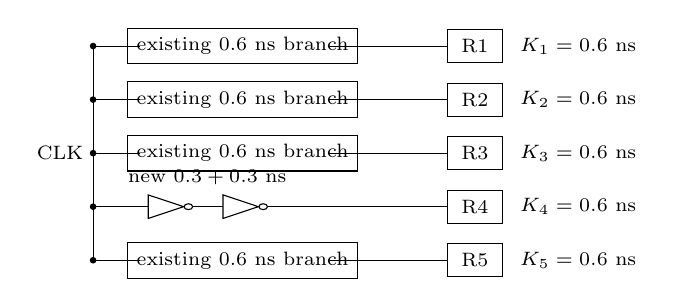
\begin{tikzpicture}[x=1cm,y=.68cm,font=\scriptsize]
\draw(0,0)--(0,4);\node[left]at(0,2){CLK};
\draw(0,4)--(.6,4);\node[draw,minimum width=2.2cm,minimum height=.28cm]at(1.9,4){existing 0.6 ns branch};\draw(3.0,4)--(4.5,4);
\node[draw,minimum width=.7cm,minimum height=.42cm]at(4.85,4){R1};\node[right]at(5.3,4){$K_{1}=0.6$ ns};\fill(0,4)circle(1.2pt);
\draw(0,3)--(.6,3);\node[draw,minimum width=2.2cm,minimum height=.28cm]at(1.9,3){existing 0.6 ns branch};\draw(3.0,3)--(4.5,3);
\node[draw,minimum width=.7cm,minimum height=.42cm]at(4.85,3){R2};\node[right]at(5.3,3){$K_{2}=0.6$ ns};\fill(0,3)circle(1.2pt);
\draw(0,2)--(.6,2);\node[draw,minimum width=2.2cm,minimum height=.28cm]at(1.9,2){existing 0.6 ns branch};\draw(3.0,2)--(4.5,2);
\node[draw,minimum width=.7cm,minimum height=.42cm]at(4.85,2){R3};\node[right]at(5.3,2){$K_{3}=0.6$ ns};\fill(0,2)circle(1.2pt);
\draw(0,1)--(.7,1);\draw(.7,0.78)--(.7,1.22)--(1.15,1)--cycle;\draw(1.21,1)circle(.055);\draw(1.27,1)--(1.65,1);\draw(1.65,0.78)--(1.65,1.22)--(2.1,1)--cycle;\draw(2.16,1)circle(.055);\draw(2.22,1)--(4.5,1);\node[above]at(1.45,1.22){new $0.3+0.3$ ns};
\node[draw,minimum width=.7cm,minimum height=.42cm]at(4.85,1){R4};\node[right]at(5.3,1){$K_{4}=0.6$ ns};\fill(0,1)circle(1.2pt);
\draw(0,0)--(.6,0);\node[draw,minimum width=2.2cm,minimum height=.28cm]at(1.9,0){existing 0.6 ns branch};\draw(3.0,0)--(4.5,0);
\node[draw,minimum width=.7cm,minimum height=.42cm]at(4.85,0){R5};\node[right]at(5.3,0){$K_{5}=0.6$ ns};\fill(0,0)circle(1.2pt);
\end{tikzpicture}\par Adverse-skew interpretation: buffer R4 only.\end{center}
The student's launch-only buffering is not a valid repair of the literal original: it makes the unbuffered R5 capture early by0.6ns and increases its setup bound to3ns. Buffer placement follows clock arrival differences, not the grade.

Hold requires $L+t_{ccq}+t_{cd}\ge K+t_{hold}$. In the balanced trees this is $t_{cd}\ge0.1$ns. The prompt gives gate propagation delays, not their contamination delays, so a physical hold guarantee cannot be deduced. Under an explicitly ideal fixed gate-delay assumption, the shortest combinational path is1ns, giving hold slack0.9ns; these conditional checks are saved separately.

\subsection*{(c) Functionally optimized NP-domino implementation}
Use Y1=VSS for its exact steady-state constant function. Generate raw dual-rail n-type dynamic nodes $d_u=\bar u$ and $d_{\bar u}=u$ with complementary XOR/XNOR pull-down minterms. Both precharge high and can only fall during evaluation. A following p-type dynamic parity stage precharges Y2 low and evaluates through either series pMOS pair $(d_u,C)$ or $(d_{\bar u},\bar C)$:
\[Y_2=\bar d_u\,\bar C+\bar d_{\bar u}\,C=u\bar C+\bar uC.\]
In the schematic, $d_u=\mathrm{raw\_xb}$ and $d_{\bar u}=\mathrm{raw\_x}$. The falling raw n-type rails monotonically enable the p-type network. True/complement A/B/C inputs must settle before evaluation; three input-complement inverters are included. Complementary clocks $\phi,\bar\phi$ are supplied externally. Weak complementary keepers retain floating states. This changes the original physical structure while preserving its Boolean outputs; the earlier timing numbers describe the original schematic, not this unsized replacement.
\newpage
% Requires TikZ only. Repeated terminal labels are electrical net names.
\providecommand{\auditmos}[4]{\begin{scope}[shift={(#1,#2)}]
\draw (0,.24)--(0,-.24);\draw (0,.20)--(.25,.20)--(.25,.5);
\draw (0,-.20)--(.25,-.20)--(.25,-.5);\draw (-.16,.23)--(-.16,-.23);
\ifnum#4=1\draw (-.26,0) circle (.06);\draw (-.75,0)--(-.32,0);
\else\draw (-.75,0)--(-.16,0);\fi
\node[anchor=east] at (-.76,0) {$#3$};\end{scope}}

\begin{center}
\begin{tikzpicture}[x=.72cm,y=.72cm,font=\scriptsize]
\auditmos{0}{0}{A}{1}
\draw (0.25,0.5)--(0.25,0.75) node[above] {$ \bar A $};
\draw (0.25,-0.5)--(0.25,-0.75) node[below] {$ V_{DD} $};
\node[anchor=west] at (0.55,0) {$M_{1}$};
\auditmos{4.8}{0}{A}{0}
\draw (5.05,0.5)--(5.05,0.75) node[above] {$ \bar A $};
\draw (5.05,-0.5)--(5.05,-0.75) node[below] {$ V_{SS} $};
\node[anchor=west] at (5.35,0) {$M_{2}$};
\auditmos{9.6}{0}{B}{1}
\draw (9.85,0.5)--(9.85,0.75) node[above] {$ \bar B $};
\draw (9.85,-0.5)--(9.85,-0.75) node[below] {$ V_{DD} $};
\node[anchor=west] at (10.15,0) {$M_{3}$};
\auditmos{14.4}{0}{B}{0}
\draw (14.65,0.5)--(14.65,0.75) node[above] {$ \bar B $};
\draw (14.65,-0.5)--(14.65,-0.75) node[below] {$ V_{SS} $};
\node[anchor=west] at (14.95,0) {$M_{4}$};
\auditmos{0}{-2.5}{C}{1}
\draw (0.25,-2)--(0.25,-1.75) node[above] {$ \bar C $};
\draw (0.25,-3)--(0.25,-3.25) node[below] {$ V_{DD} $};
\node[anchor=west] at (0.55,-2.5) {$M_{5}$};
\auditmos{4.8}{-2.5}{C}{0}
\draw (5.05,-2)--(5.05,-1.75) node[above] {$ \bar C $};
\draw (5.05,-3)--(5.05,-3.25) node[below] {$ V_{SS} $};
\node[anchor=west] at (5.35,-2.5) {$M_{6}$};
\auditmos{9.6}{-2.5}{\phi}{0}
\draw (9.85,-2)--(9.85,-1.75) node[above] {$ \mathrm{en} $};
\draw (9.85,-3)--(9.85,-3.25) node[below] {$ V_{SS} $};
\node[anchor=west] at (10.15,-2.5) {$M_{7}$};
\auditmos{14.4}{-2.5}{\phi}{1}
\draw (14.65,-2)--(14.65,-1.75) node[above] {$ \mathrm{raw\_x} $};
\draw (14.65,-3)--(14.65,-3.25) node[below] {$ V_{DD} $};
\node[anchor=west] at (14.95,-2.5) {$M_{8}$};
\auditmos{0}{-5}{A}{0}
\draw (0.25,-4.5)--(0.25,-4.25) node[above] {$ \mathrm{raw\_x} $};
\draw (0.25,-5.5)--(0.25,-5.75) node[below] {$ \mathrm{raw\_x\_u0} $};
\node[anchor=west] at (0.55,-5) {$M_{9}$};
\auditmos{4.8}{-5}{B}{0}
\draw (5.05,-4.5)--(5.05,-4.25) node[above] {$ \mathrm{raw\_x\_u0} $};
\draw (5.05,-5.5)--(5.05,-5.75) node[below] {$ \mathrm{en} $};
\node[anchor=west] at (5.35,-5) {$M_{10}$};
\auditmos{9.6}{-5}{\bar A}{0}
\draw (9.85,-4.5)--(9.85,-4.25) node[above] {$ \mathrm{raw\_x} $};
\draw (9.85,-5.5)--(9.85,-5.75) node[below] {$ \mathrm{raw\_x\_u1} $};
\node[anchor=west] at (10.15,-5) {$M_{11}$};
\auditmos{14.4}{-5}{\bar B}{0}
\draw (14.65,-4.5)--(14.65,-4.25) node[above] {$ \mathrm{raw\_x\_u1} $};
\draw (14.65,-5.5)--(14.65,-5.75) node[below] {$ \mathrm{en} $};
\node[anchor=west] at (14.95,-5) {$M_{12}$};
\auditmos{0}{-7.5}{\mathrm{raw\_x}}{1}
\draw (0.25,-7)--(0.25,-6.75) node[above] {$ \mathrm{kx} $};
\draw (0.25,-8)--(0.25,-8.25) node[below] {$ V_{DD} $};
\node[anchor=west] at (0.55,-7.5) {$M_{13}$};
\auditmos{4.8}{-7.5}{\mathrm{raw\_x}}{0}
\draw (5.05,-7)--(5.05,-6.75) node[above] {$ \mathrm{kx} $};
\draw (5.05,-8)--(5.05,-8.25) node[below] {$ V_{SS} $};
\node[anchor=west] at (5.35,-7.5) {$M_{14}$};
\auditmos{9.6}{-7.5}{\mathrm{kx}}{1}
\draw (9.85,-7)--(9.85,-6.75) node[above] {$ \mathrm{raw\_x} $};
\draw (9.85,-8)--(9.85,-8.25) node[below] {$ V_{DD} $};
\node[anchor=west] at (10.15,-7.5) {$M_{15}$ (weak)};
\auditmos{14.4}{-7.5}{\phi}{1}
\draw (14.65,-7)--(14.65,-6.75) node[above] {$ \mathrm{raw\_xb} $};
\draw (14.65,-8)--(14.65,-8.25) node[below] {$ V_{DD} $};
\node[anchor=west] at (14.95,-7.5) {$M_{16}$};
\auditmos{0}{-10}{\bar A}{0}
\draw (0.25,-9.5)--(0.25,-9.25) node[above] {$ \mathrm{raw\_xb} $};
\draw (0.25,-10.5)--(0.25,-10.75) node[below] {$ \mathrm{raw\_xb\_u0} $};
\node[anchor=west] at (0.55,-10) {$M_{17}$};
\auditmos{4.8}{-10}{B}{0}
\draw (5.05,-9.5)--(5.05,-9.25) node[above] {$ \mathrm{raw\_xb\_u0} $};
\draw (5.05,-10.5)--(5.05,-10.75) node[below] {$ \mathrm{en} $};
\node[anchor=west] at (5.35,-10) {$M_{18}$};
\auditmos{9.6}{-10}{A}{0}
\draw (9.85,-9.5)--(9.85,-9.25) node[above] {$ \mathrm{raw\_xb} $};
\draw (9.85,-10.5)--(9.85,-10.75) node[below] {$ \mathrm{raw\_xb\_u1} $};
\node[anchor=west] at (10.15,-10) {$M_{19}$};
\auditmos{14.4}{-10}{\bar B}{0}
\draw (14.65,-9.5)--(14.65,-9.25) node[above] {$ \mathrm{raw\_xb\_u1} $};
\draw (14.65,-10.5)--(14.65,-10.75) node[below] {$ \mathrm{en} $};
\node[anchor=west] at (14.95,-10) {$M_{20}$};
\auditmos{0}{-12.5}{\mathrm{raw\_xb}}{1}
\draw (0.25,-12)--(0.25,-11.75) node[above] {$ \mathrm{kxb} $};
\draw (0.25,-13)--(0.25,-13.25) node[below] {$ V_{DD} $};
\node[anchor=west] at (0.55,-12.5) {$M_{21}$};
\auditmos{4.8}{-12.5}{\mathrm{raw\_xb}}{0}
\draw (5.05,-12)--(5.05,-11.75) node[above] {$ \mathrm{kxb} $};
\draw (5.05,-13)--(5.05,-13.25) node[below] {$ V_{SS} $};
\node[anchor=west] at (5.35,-12.5) {$M_{22}$};
\auditmos{9.6}{-12.5}{\mathrm{kxb}}{1}
\draw (9.85,-12)--(9.85,-11.75) node[above] {$ \mathrm{raw\_xb} $};
\draw (9.85,-13)--(9.85,-13.25) node[below] {$ V_{DD} $};
\node[anchor=west] at (10.15,-12.5) {$M_{23}$ (weak)};
\auditmos{14.4}{-12.5}{\bar\phi}{1}
\draw (14.65,-12)--(14.65,-11.75) node[above] {$ \mathrm{ep} $};
\draw (14.65,-13)--(14.65,-13.25) node[below] {$ V_{DD} $};
\node[anchor=west] at (14.95,-12.5) {$M_{24}$};
\auditmos{0}{-15}{\bar\phi}{0}
\draw (0.25,-14.5)--(0.25,-14.25) node[above] {$ \mathrm{y2} $};
\draw (0.25,-15.5)--(0.25,-15.75) node[below] {$ V_{SS} $};
\node[anchor=west] at (0.55,-15) {$M_{25}$};
\auditmos{4.8}{-15}{\mathrm{raw\_xb}}{1}
\draw (5.05,-14.5)--(5.05,-14.25) node[above] {$ \mathrm{ep} $};
\draw (5.05,-15.5)--(5.05,-15.75) node[below] {$ \mathrm{yp0} $};
\node[anchor=west] at (5.35,-15) {$M_{26}$};
\auditmos{9.6}{-15}{C}{1}
\draw (9.85,-14.5)--(9.85,-14.25) node[above] {$ \mathrm{yp0} $};
\draw (9.85,-15.5)--(9.85,-15.75) node[below] {$ \mathrm{y2} $};
\node[anchor=west] at (10.15,-15) {$M_{27}$};
\auditmos{14.4}{-15}{\mathrm{raw\_x}}{1}
\draw (14.65,-14.5)--(14.65,-14.25) node[above] {$ \mathrm{ep} $};
\draw (14.65,-15.5)--(14.65,-15.75) node[below] {$ \mathrm{yp1} $};
\node[anchor=west] at (14.95,-15) {$M_{28}$};
\auditmos{0}{-17.5}{\bar C}{1}
\draw (0.25,-17)--(0.25,-16.75) node[above] {$ \mathrm{yp1} $};
\draw (0.25,-18)--(0.25,-18.25) node[below] {$ \mathrm{y2} $};
\node[anchor=west] at (0.55,-17.5) {$M_{29}$};
\auditmos{4.8}{-17.5}{\mathrm{y2}}{1}
\draw (5.05,-17)--(5.05,-16.75) node[above] {$ \mathrm{ky} $};
\draw (5.05,-18)--(5.05,-18.25) node[below] {$ V_{DD} $};
\node[anchor=west] at (5.35,-17.5) {$M_{30}$};
\auditmos{9.6}{-17.5}{\mathrm{y2}}{0}
\draw (9.85,-17)--(9.85,-16.75) node[above] {$ \mathrm{ky} $};
\draw (9.85,-18)--(9.85,-18.25) node[below] {$ V_{SS} $};
\node[anchor=west] at (10.15,-17.5) {$M_{31}$};
\auditmos{14.4}{-17.5}{\mathrm{ky}}{0}
\draw (14.65,-17)--(14.65,-16.75) node[above] {$ \mathrm{y2} $};
\draw (14.65,-18)--(14.65,-18.25) node[below] {$ V_{SS} $};
\node[anchor=west] at (14.95,-17.5) {$M_{32}$ (weak)};
\end{tikzpicture}
\end{center}
\noindent\textbf{Q6(c),32MOS NP parity implementation}. $Y_1$ is tied to $V_{SS}$. The two N-type raw rails begin high and only fall; the P-type output begins low and only rises. $Y_2=A\oplus B\oplus C$. Three input inverters and weak feedback keepers are included. The N-stage raw rails connect directly to the P-stage gates; the side inverters only control keepers.
 Identically named terminals are connected. All nMOS bodies use $V_{SS}$ and all pMOS bodies use $V_{DD}$.

All eight words are checked under precharge/evaluate conditions. It is an ideal functional NP-domino design without unprovided physical delay or power claims.

\subsection*{(d) Logic masking and soft errors}
The classroom comparison favors R5 as more vulnerable to combinational logic faults: its parity path propagates every single input-bit error, while the R4 path masks many disturbances. For example, flipping internal u flips Y2 for all8 input words, but changes Y1 only for ABC=111 (1of8). This is a specific functional masking argument, not a rule that counting more gates always reduces errors.

Assuming equal register cells/exposure and comparable electrical/timing masking, that supports a higher combinational-error contribution at R5. The actual total soft-error rate also includes direct register strikes, pulse attenuation/capture windows, capacitance, layout and radiation conditions; none are specified, so an unconditional numerical SER ranking is not determined.

\section*{Source comparison, checks and reproduction}
Q1's useful mechanisms are retained with corrected physical explanations. Q2's recurrence is independently implemented with explicit shared multioutput structure. Q3 repairs the exact middle-stage clock-phase/polarity issue and enumerates valid sharing-only states. Q4 separates fixed-C grading convention from the literal capacitive-load inconsistency. Q5 includes all14 layout crossings. Q6 preserves the original NOR/XOR gates and both approved skew readings, corrects buffer placement, and gives a functional NP implementation.

Run \texttt{python verify\_dynamic\_schmitt.py} and \texttt{python verify\_logic\_timing.py}. Saved CSV/JSON files give ideal-graph, capacitance and timing evidence. No process model is needed. Both reports are standalone pdfLaTeX sources; every figure uses editable TikZ and no scan images. The retained question allocations sum to110points, as printed.

\section*{Primary technical references}
\begin{enumerate}[leftmargin=7mm,itemsep=4pt]
\item Texas Instruments, \href{https://www.ti.com/lit/pdf/slya014}{Latch-Up, ESD, and Other Phenomena}: parasitic PNPN action and guard-ring/body-contact mitigation.
\item Synopsys, \href{https://www.synopsys.com/articles/finfet-design.html}{FinFET Design Insights and Reliability}, aging section: NBTI threshold degradation under voltage, temperature and duration stress; historical roadmap predictions are not used.
\item MIT6.374, \href{https://ocw.mit.edu/courses/6-374-analysis-and-design-of-digital-integrated-circuits-fall-2003/b4b0ba298ce3c93e19f24215304850c5_ps3_03.pdf}{Problem Set3}: dynamic-logic charge-sharing and clock-cycle analysis. Circuit derivations here follow this paper's actual supplied topology.
\end{enumerate}
\end{document}
